\documentclass{article}

\usepackage{amsmath, amsthm, amssymb, amsfonts}
\usepackage{thmtools}
\usepackage{graphicx}
\usepackage{setspace}
\usepackage{geometry}
\usepackage{float}
\usepackage{hyperref}
\usepackage[utf8]{inputenc}
\usepackage[spanish]{babel}
\usepackage{framed}
\usepackage[dvipsnames]{xcolor}
\usepackage{tcolorbox}

\graphicspath{ {./images/} }

\colorlet{LightGray}{White!90!Periwinkle}
\colorlet{LightOrange}{Orange!15}
\colorlet{LightGreen}{Green!15}

\newcommand{\HRule}[1]{\rule{\linewidth}{#1}}

\declaretheoremstyle[name=Ejemplo,]{thmsty}
\declaretheorem[style=thmsty,numberwithin=subsection]{ejemplo}

\declaretheoremstyle[name=Theorem,]{thmsty}
\declaretheorem[style=thmsty,numberwithin=section]{theorem}
\tcolorboxenvironment{theorem}{colback=LightGray}

\declaretheoremstyle[name=Proposition,]{prosty}
\declaretheorem[style=prosty,numberlike=theorem]{proposition}
\tcolorboxenvironment{proposition}{colback=LightOrange}

\declaretheoremstyle[name=Principle,]{prcpsty}
\declaretheorem[style=prcpsty,numberlike=theorem]{principle}
\tcolorboxenvironment{principle}{colback=LightGreen}

\setstretch{1.2}
\geometry{
    textheight=9in,
    textwidth=5.5in,
    top=1in,
    headheight=12pt,
    headsep=25pt,
    footskip=30pt
}

% ------------------------------------------------------------------------------

\begin{document}

% ------------------------------------------------------------------------------
% Cover Page and ToC
% ------------------------------------------------------------------------------

\title{ \normalsize \textsc{}
		\\ [2.0cm]
		\HRule{1.5pt} \\
		\LARGE \textbf{\uppercase{Apunte Olimpíadas Ñandú}
		\HRule{2.0pt} \\ [0.6cm] \vspace*{10\baselineskip}}
		}
\date{}
\author{\textbf{Autor} \\ 
		Ignacio Cuevas \\
		Córdoba, Argentina \\
		2023}

\maketitle
\newpage

\tableofcontents
\newpage

\section{Introducción a las Competencias}

\subparagraph*{}
\begin{small}
En este apunte vamos a estudiar los diferentes tipos de problemas que nos podemos encontrar en la Olimpíada de Matemáticas Ñandú (Tercer nivel) y vamos a aprender algunas herramientas que nos serán útil para resolver cada uno de los problemas.
\end{small}

\newpage

\section{La Competencia}

\subparagraph*{}
\begin{small}
La competencia consta de 3 ejercicios:
\begin{enumerate}
	\item El primer ejercicio de Álgebra
	\item El segundo de Geometría
	\item Y el tercero de Conteo
\end{enumerate}
Ahora pasaremos a explicar cada uno de ellos.
\end{small}

\subsection{Álgebra}
\begin{small}
En este primer tipo de ejercicios nos vamos a encontrar problemas donde nos presentan un tipo de objeto (por ejemplo, verduras), y ciertos valores de ellos (por ejemplo, su precio), ya sea el objeto individual o sumas de varios. Veamos un ejemplo para que quede más claro.
\\
\end{small}

\begin{ejemplo}
En las bolsas A, B y C hay en total 200 caramelos. En la bolsa B hay 20 más que
en la A, en la bolsa C hay 61 más que en la B. ¿Cuántos caramelos hay en la bolsa C?
\end{ejemplo}

\begin{ejemplo}
En el colegio hay 1360 alumnos inscriptos. De los alumnos inscriptos, $\frac{3}{5}$ se anotaron en el turno mañana. De los alumnos del turno mañana, $\frac{1}{4}$ van al jardín, $\frac{2}{3}$ van a la primaria y los demás van a la secundaria. ¿Cuántos alumnos van a la secundaria en el turno mañana?
\end{ejemplo}

\subsection{Geometria}
\begin{small}
Este segundo ejercicio es de geometría, es decir, nos vamos a encontrar con ejercicios que involucran figuras, lados, ángulos.
El dibujo puede estar dado en el ejercicio, o pueden dar las características para que uno lo grafique. Estos dibujos muchas veces tienen puntos clave representados con letras.
Los datos que nos dan pueden ser las medidas de algunos lados, ángulos, perímetros, áreas, etc.
\\ \\
\end{small}

\begin{ejemplo}
ABCD es un rectángulo,
AB = 3BC;
M es punto medio de AB;
N es punto medio de AD;
P es punto medio de CD;
O es el punto medio del segmento MP.
El perímetro de AMPD es de 80cm.
¿Cuál es el perímetro de AMON?
¿Cuál es el área de BCPO?

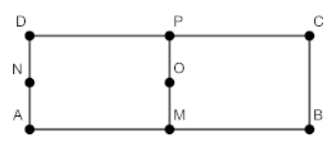
\includegraphics[scale=0.6]{geometry-example-1}
\\
\\
\end{ejemplo}

\begin{ejemplo}
En la figura:
ABC es un triángulo equilátero,
EFGH es un rectángulo,
CDE es un triángulo rectángulo,
F es punto medio de AB,
G es punto medio de BC,
DE = AB,
Perímetro de ABC = 96cm.
¿Cuál es el área de EFGH?
¿Cuál es el perímetro de CDFG?
¿Cuál es el área de ABCD?
¿Cuál es el área de CDG?

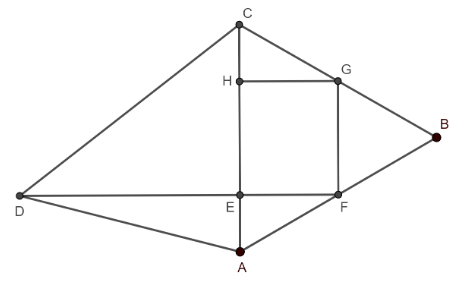
\includegraphics[scale=0.6]{geometry-example-2}
\end{ejemplo}

\subsection{Conteo}
\begin{small}
Este último ejercicio, como bien dice su nombre, tenemos que contar cosas. Pueden ser números en un cierto rango que cumplen ciertas propiedades, formas de hacer determinada cosa, u otras cosas. Como datos nos van a dar el problema y sus restricciones.
\\
\\
\end{small}

\begin{ejemplo}
Luis come, en total, 5 chocolatines en la semana, de lunes a viernes.
Puede comer 2 chocolatines, 1 chocolatín o ningún chocolatín en el mismo día.
En esta tabla anota cuántos chocolatines come cada día.
¿De cuántas maneras distintas puede completar la tabla?
Explica cómo las contaste.
\\
\\
\end{ejemplo}

\begin{ejemplo}
Aníbal y Beto están en el equipo de pingpong.
Martín, Nicolás, Oscar y Pablo están en el equipo de tenis.
Ramón, Santiago y Tomás están en el equipo de natación.
Entre estos deportistas deben elegir un grupo de 5 para hacer un viaje.
Si en el grupo debe haber por lo menos un representante de cada deporte,
¿de cuántas maneras distintas puede hacerse la elección?
Explica cómo las contaste.

\end{ejemplo}

\newpage

\section{Álgebra}
\begin{small}
En este primer módulo vamos a ver que herramientas nos serán de gran utilidad para resolver ejercicios del primer tipo mencionado en la introducción.
Nos vamos a enfocar en:
\begin{enumerate}
	\item Manejar bien las unidades y los números.
	\item Entender la noción de ecuación.
	\item Apender a resolver ecuaciones.
	\item Interpretar un problema para armar ecuaciones.
\end{enumerate}
\end{small}

\subsection{Manejo de números}
\begin{small}
Antes de largarnos a aprender ecuaciones es importante que entendamos que hay diferentes formas de representar los números. Es decir que podemos ver dos numeros con representaciones distintas y que valen lo mismo.
\end{small}

\subsubsection*{Números enteros y reales}
\begin{small}
Los numeros enteros representan cosas, como bien dice su nombre, enteras. Podemos decir \textit{1, 2, 3 autos}, pero no podemos decir \textit{un auto y medio}, o \textit{3.14 autos}. Para esta otra representacion existen los números reales, por ejemplo podemos decir, \textit{1.5 litros de leche}, o \textit{11.86 cm}.
Cada uno de estos tipos tienen propiedades que no vamos a ver en esta sección, sino en la de \textit{Conteo}.
\end{small}

\subsubsection*{Fracciones}
\begin{small}
Las fracciones son formas de representar números reales con números enteros. Muchas veces se usan para llegar a un resultado más exacto o para no trabajar con números con decimales (estos pueden ser más difíciles de manipular). Un número fraccionario consta de dos partes, el numerador (arriba) y el denominador (abajo),
\[\frac{x}{y}=x:y=x/y\]
Por ejemplo, podemos leer la siguiente fracción de varias formas $\frac{3}{4}$, tres cuartos, tres dividido cuatro, tres sobre cuatro, tres partes de cuatro, 0.75, entre muchas otras formas.
\\
\end{small}

\begin{normalsize}
\begin{center}
\textbf{Operaciones con fracciones}
\end{center}
\end{normalsize}

\begin{small}
\textbf{Suma y resta:} Hay dos tipos de sumas, con mismo denominador y con distinto denominador.
Con mismo denominador se suman directamente los numeradores.
\[\frac{x}{d}+\frac{y}{d}=\frac{x+y}{d}\]
\[\frac{x}{d}-\frac{y}{d}=\frac{x-y}{d}\]

Con distinto denominador:
\begin{itemize}
	\item Denominador: se multiplican los denominadores.
	\item Numerador: Se multiplican numerador con denominador contrario y se suman.
\end{itemize}
Veamos la fórmula:
\[\frac{x}{a}+\frac{y}{b}=\frac{xb+ya}{ab}\]

\textbf{Producto:} se multiplica numerador con numerador, y denominador con denominador.
\[\frac{x}{a}\cdot\frac{y}{b}=\frac{xy}{ab}\]

\textbf{División:} en el numerador del resultado se coloca el producto entre el primer numerador con el denominador del segundo, y en el denominador del resultado el producto entre denominador del primero con el numerador del segundo.
\[\frac{x}{a}\cdot\frac{y}{b}=\frac{xb}{ay}\]\\

\textbf{Nota:} Cuando operamos entre fracciones y números enteros, es útil ver que un número entero tiene denominador 1. Por ejemplo, $4=\frac{4}{1}$\\

\textbf{Nota:} Si multiplicamos o dividimos dos numeros inversos, es decir que el numerador de uno es el denominador del otro y viceversa, el resultado es 1. Por ejemplo, $\frac{2}{5}\cdot\frac{5}{2}=1$, lo mismo con un entero, $4\cdot\frac{1}{4}=\frac{4}{1}\cdot\frac{1}{4}=1$\\

\textbf{Definición:} Decimos que el número inverso de $\frac{a}{b}$ es $\frac{b}{a}$\\

\textbf{Observación:} Podemos decir que dividir $\frac{a}{b}$ es lo mismo que multiplicar $a$ por el inverso de $b$. $\frac{a}{b}=a\cdot\frac{1}{b}$\\
\end{small}

\subsubsection*{Porcentajes}
\begin{small}
Los porcentajes se aplican a una cantidad, por ejemplo \textit{el 50\% de las manzanas}, o \textit{se aumento un 110\% del precio original}.
Cada porcentaje se puede representar como un número real.
Por ejemplo,
\begin{itemize}
	\item El 25\% de B, es lo mismo que $0.25B$, o $\frac{1}{4}B$
	\item El 110\% de C, es lo mismo que $1.1C$, o $\frac{11}{10}C$
	\item El 10\% menos de D, es lo mismo que $D-0.1D=0.9D$
\end{itemize}
\end{small}

\subsection{Noción de ecuacion}
\begin{small}
Una ecuación es una igualdad. Consta de tres partes, dos expresiones y un símbolo de igual ($=$) entre ellas.
\[expr1=expr2\]
Entonces, como tenemos que mantener siempre la igualdad, si sumamos $4$ de un lado, tenemos que sumar $4$ del otro.
\[expr1+4=expr2+4\]
Podemos ver un ejemplo concreto,
\[(3+2)=5\]
\[(3+2)+4=5+4\]
pero,
\[(3+2)+2\neq5+4\]
Lo mismo pasa con las demas operaciones, si restamos en un lado, restamos lo mismo en el otro, si multiplicamos o dividimos de un lado, hacemos lo mismo del otro.
\end{small}

\subsection{Resolución de ecuaciones}
\begin{small}
Que pasa cuando en una ecuación, que antes vimos que es una igualdad, hay una incógnita (o valor desconocido). Cómo podemos hacer para obtener su/sus valores posibles. Eso es lo que vamos a estar viendo en esta parte.

Primero, que es una incógnita y cómo podemos representar una ecuación con incógnitas. Una incógnita es un valor desconocido que buscamos encontrar. En general, esta se representa con letras. Por ejemplo, 
\[2x=4\]
\[6b+7=13\]
\[\frac{3+k}{2}=8\]
\[1.1m-\frac{2m}{3}=1.25\]
\end{small}

\subsubsection*{Cómo resolver ecuaciones con una incógnita}
\begin{small}
Para resolver una ecuación con una incógnita tenemos que aplicar operaciones inteligentemente (recordemos que aplicamos la misma operación a ambos lados), para que nos quede nuestra incógnita sola (o despejada) en uno de los lados.
Un par de aclaraciones antes de ver un ejemplo.
\begin{itemize}
	\item Es lo mismo escribir $x$ que $1\cdot x$, es lo mismo escribir $2x$ que $2\cdot x$
	\item No podemos sumar $x+4$, simplemente dejamos la expresión como esta. Tenemos que sumar números con números, e incógnitas del mismo tipo. (Nota: si podemos multiplicar).
	
	Por ejemplo, $5x+2x=7x$ y $2x+7+3x+1=5x+8$.
\end{itemize}

Ahora veamos un ejemplo con los pasos a seguir para resolver una ecuación con una incógnita,

\begin{align}
2x+7 &= 10\\2x+7-7&=10-7\\2x+0&=10-7\\2x&=3\\\frac{2x}{2}&=\frac{3}{2}\\x&=\frac{3}{2}
\end{align}

Y listo, ya obtuvimos el valor de $x=\frac{3}{2}$

Veamos esto paso por paso,
\begin{enumerate}
	\item Planteamos la ecuación.
	\item Como buscamos \textit{despejar x}, nos conviene restar \textit{7} en ambos lados.
	\item Resolvemos el lado izquierdo (recordemos las aclaraciones antes mencionadas).
	\item Resolvemos el lado derecho.
	\item Ahora nos conviene dividir ambos lados por \textit{2}, ya que $\frac{2}{2}=1$ y $1x=x$
	\item Finalmente resolvemos el lado izquierdo, ya que en el derecho no queda nada por resolver y vemos que nos queda la \textit{x despejada}.
\end{enumerate}
\end{small}

\subsubsection*{Ejercicios de práctica}
\begin{small}
\begin{enumerate}
	\item $6x-4=26$
	\item $12x+8=5x+36$
	\item $3(2x-6)=2(5x+3)$
	\item $\frac{4x+5}{5}=\frac{x+17}{3}$
\end{enumerate}
\end{small}

\subsection{Cómo interpretar un problema}
\begin{small}
\textbf{Importante:} Para interpretar y plantear un problema con facilidad y rapidez, es necesario de mucha práctica.

La resolución de problemas de matemáticas recorre cuatro fases:
\begin{enumerate}
	\item Comprender el problema
	\item Elaborar un plan para resolverlo
	\item Ejecutar el plan
	\item Comprobar que la respuesta es correcta
\end{enumerate}

Veamos varios ejemplos para que se entienda.
\\
\end{small}

\begin{ejemplo}
El doble de un número es igual a 10.

\begin{enumerate}
	\item El problema es, encontrar un número tal que multiplicado por 2 es 10.
	\item Podemos plantear la siguiente ecuación: $2n=10$
	\item Resolvemos la ecuación.
		\begin{align}
		2n&=10\nonumber\\
		\frac{2n}{2}&=\frac{10}{2}\nonumber\\
		n&=5\nonumber
		\end{align}
	\item Comprobamos que este bien. $2\cdot5=10$
\end{enumerate}

\end{ejemplo}

\begin{ejemplo}
La mitad de un número más 5 es igual a 8.

\begin{enumerate}
	\item Acá es un poco diferente, pero sabemos que la mitad de un número es lo mismo que dividir un número por 2. El problema que nos plantean es, encontrar un número tal que, si lo dividimos por 2 ($\frac{k}{2}$) y a ese resultado le sumamos 5 ($\frac{k}{2}+5$), obtenemos 8 ($\frac{k}{2}+5=8$).
	\item Planteemos la ecuación: $\frac{k}{2}+5=8$
	\item Resolvamos para k.
	\begin{align}
	\frac{k}{2}+5&=8\nonumber\\
	\frac{k}{2}+5-5&=8-5\nonumber\\
	\frac{k}{2}&=3\nonumber\\
	\frac{k}{2}\cdot2&=3\cdot2\nonumber\\
	k\cdot1&=6\nonumber
	\end{align}
	\item Comprobamos que este bien. $\frac{6}{2}+5=3+5=8$
\end{enumerate}

\end{ejemplo}

\begin{ejemplo}
En el kiosco, 1 gaseosa cuesta \$12 y 1 jugo cuesta \$7.
Compré 2 gaseosas, 1 jugo y 3 paquetes de galletitas. Pagué \$49 en total.
¿Cuál es el precio de cada paquete de galletitas?

\begin{enumerate}
	\item Los datos que nos dan son los precios de algunos productos, y sabemos que la suma de cierta cantidad de productos da \$49. Nuestra incógnita en este caso es el precio de las galletitas.
	\item Antes de empezar veamos lo siguiente, llamemos G=gaseosa, J=jugo, M=galletitas \textit{(de masitas, no uso G de galletitas porque ya G significa gaseosa)}:
		\begin{itemize}
			\item $1\cdot G=G=12$, una gaseosa cuesta \$12.
			\item $1\cdot J=J=7$, un jugo \$7.
			\item $M=?$
		\end{itemize}
	Ahora si podemos plantear la ecuación. Tenemos que decir que 2 gaseosas, 1 jugo y 3 paquetes de galletitas cuestan \$49, entonces:
	\[2G+J+3M=49\]
	Pero algunos valores ya los tenemos,
	\[2\cdot12+7+3M=49\]
	\[24+7+3M=49\]
	\[31+3M=49\]
	\item Una vez que sustituimos los valores correspondientes, procedemos a resolver la ecuación:
		\begin{align}
		31+3M&=49\nonumber\\
		31+3M-31&=49-31\nonumber\\
		3M&=18\nonumber\\
		\frac{3M}{3}&=\frac{18}{3}\nonumber\\
		M&=6\nonumber
		\end{align}
	\item Veamos que se cumple lo primero que planteamos con el valor obtenido:
	\[2G+J+3M=49\]
	\[2\cdot12+7+3\cdot6=49\]
	\[24+7+18=49\]
	\[49=49\]
\end{enumerate}

\end{ejemplo}

\begin{ejemplo}
De los socios del club $\frac{7}{8}$ se anotaron para ir a la cena de fin de año, pero $\frac{1}{4}$ de los anotados no fueron a la cena. Si había 315 socios en la cena, ¿cuántos socios se anotaron para la cena?, ¿cuántos socios tiene el club?
\\ \\
En principio, este problema parece tener pocos datos, pero veremos que son suficientes.
\begin{enumerate}
	\item El primer dato que tenemos claro es que hay 315 socios en la cena. Ahora, ¿cuál es el valor desconocido? Es la cantidad de socios totales del club, pues con ese valor podemos calcular fácilmente la cantidad de anotados para la cena, ($\frac{7}{8}$ del total).
	
Llamemos $S$ a la cantidad total de socios que tiene el club. Sabemos que de \textbf{todos} los socios del club, se anotaron $\frac{7}{8}$ de ellos. Más formalmente $\frac{7}{8}S$. Y de esa cantidad, $\frac{1}{4}$ no fue a la cena, o dicho de otro modo, $\frac{3}{4}$ si fueron.

	\item Entonces, si ya \textit{"conocemos"} la porción de personas que fueron a la cena, podemos plantear la ecuación:
	\[(\frac{7}{8}S)(\frac{3}{4})=315\]
	\item Resolvamos para $S$.
	\begin{align}
	(\frac{7}{8}S)(\frac{3}{4})&=315\nonumber\\
	\frac{21}{32}S&=315\nonumber\\
	(\frac{21}{32}S)\cdot\frac{32}{21}&=315\cdot\frac{32}{21}\nonumber\\
	S&=\frac{10080}{21}\nonumber\\
	S&=480\nonumber
	\end{align}
	Ya conocemos el valor de $S$, que habiamos dicho que era el total de socios del club. Ahora nos falta ver cuántos socios se anotaron para la cena, que en un principio sabíamos que era $\frac{7}{8}S=\frac{7}{8}\cdot480=420$. Entonces la respuesta es: la cantidad total de socios que tiene el club son 480, de esos, 420 se anotaron para ir a la cena. Pregunta: ¿Cuántos no fueron a la cena?
	\item Comprobamos que esté bien. $(\frac{7}{8}S)(\frac{3}{4})=(\frac{7}{8}\cdot480)(\frac{3}{4})=420\cdot(\frac{3}{4})=\frac{1260}{4}=315$
\end{enumerate}

\end{ejemplo}

\end{document}